\section{Definicion de IA}

\begin{figure}
  \centering
  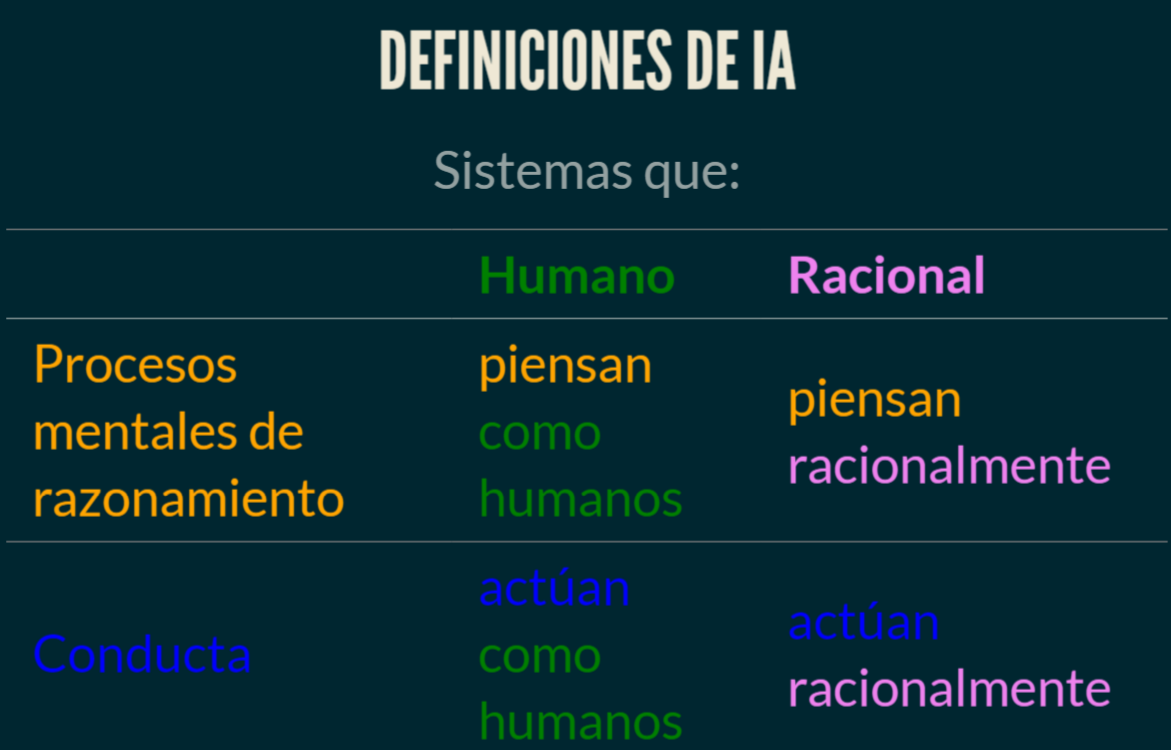
\includegraphics[width=16cm, scale=1]{Images/Imagenes/cuadro1.png}
  \caption{Definiciones de IA}
  \label{fig:marcado}
\end{figure}

\begin{itemize}
  \item \textbf{Piensan como humanos:} Requiere de teorías científicas de las actividades internas del cerebro. Para lograrlo hay que determinar como es que piensan los humanos.
  \item \textbf{Piensan racionalmente:} ir al cap 1 de \cite{sabharwal2011s}
  \item \textbf{Actúan como humanos: }El modelo es el hombre; el objetivo es construir un sistema que se haga pasar por un humano.
  
  Turing propone un Test operacional para el funcionamiento inteligente las capacidades necesarias son:
  \begin{itemize}
    \item Procesamiento de lenguaje natural
    \item Representación del conocimiento
    \item Razonamiento
    \item Aprendizaje
  \end{itemize}
  El Test consiste en un juez realizando preguntas a dos participantes (X e Y) que no puede ver: un hombre y una mujer. El juez debe averiguar por medio de preguntas quien es el hombre y quien la mujer. Los participantes pueden mentir o tratar de engañar al juez
  \item \textbf{Actúan racionalmente (este es el que nos interesa):} El comportamiento racional hace referencia a realizar la acción correcta. Es decir aquello que se espera maximice la meta a alcanzar dada la información disponible
\end{itemize}

\textbf{Agente: }Un agente es una entidad que percibe y actúa. Abstractamente un agente es una función desde historias de percepciones a acciones:

\begin{equation}
  f: P* \rightarrow A 
\end{equation}

Para toda clase de ambientes y tareas buscamos el agente con la mejor perfomance

\textbf{IA fuerte vs Debil }
\begin{itemize}
  \item \textbf{IA fuerte: }Una maquina que piense debera tener conciencia y mente real
  \item \textbf{IA débil: }Las maquinas podrían actuar como si ellas fueran inteligentes
\end{itemize}

\textbf{Inteligencia artificial vs sintética}
\begin{itemize}
  \item \textbf{Artificial: }Hecho por el hombre. Sugiere que es algo de calidad diferente a lo natural. Por ejemplo lago artificial brazo artificial.
  \item \textbf{Sintético: }Producto obtenido por procedimientos mecánicos electrónicos o industriales y que imita otro producto natural. Por ejemplo césped sintético  
\end{itemize}

\subsection{Agentes}
\todo[inline]{Esta seccion hay que sabersela de memoria se arrastra hasta el final de la carrera}
Un agente racional es aquel que hace las acciones correctas. Una accion correcta es aquella que causa que el agente sea mas exitoso.
\begin{itemize}
  \item Una \textbf{secuencia de acciones} afectan al ambiente que pasa por una secuencia de estados. Por ejemplo cuando moves una pieza jugando al ludo el ambiente es el tablero y tu acción de mover una pieza modifico la configuración de este
  \item \textbf{Medida de performance} criterio objetivo que establece cuan exitoso es el comportamiento del agente. Evalúa cuan deseable es la secuencia de estados del ambiente generados por la secuencia de acciones del agente
\end{itemize}

Las medidas de performance se diseñan de acuerdo a loq ue uno realmente \textbf{quiere en el ambiente} en vez de considerar la forma en que uno piensa que el agente se debería comportar

\textbf{Racionalidad en un agente racional: }en un momento dado depende de:
\begin{itemize}
  \item La medida de performance que define un criterio de éxito
  \item El conocimiento a priori del ambiente
  \item Las acciones que el agente puede ejecutar
  \item La secuencia de percepciones del agente hasta el momento
  \item Para cada posible secuencia de percepciones un agente racional elige la acción que maximiza el valor esperado de la medida de performance (osea la acción que lo hace mas exitoso) esto lo averigua basándose en la evidencia provista por la secuencia de percepciones y el conocimiento predefinido que el agente tiene
\end{itemize}

\textbf{Agente omnisciente: }es aquel que conoce el resultado real de sus acciones y puede actuar de a cuerdo a ello. Esta es imposible en la realidad ya que $Racionalidad \neq Clarividencia$. El agente racional no requiere omnisciencia porque la elección racional depende de la secuencia de percepciones

\textbf{Como trabaja el agente racional:}
\begin{itemize}
  \item Explora: reúne información antes de elegir la acción adecuada. Ejemplo: Si tenes un robot que tiene que cruzar la calle tiene que mirar a los dos lados para saber cuando cruzar y que no se la den
  \item Autonomía: Toma decisiones en forma \textbf{independiente}. Sus decisiones y sus acciones están bajo su propio control. Tiene sus propias creencias deseos e intenciones es decir no es sirviente de otros (hace la que le pinta en función a lo que sabe). Si un agente confía en el conocimiento a priori de su diseñador en vez de en sus percepciones entonces se dice que le falta autonomía 
\end{itemize}

\subsection*{Tipos de agentes}
\subsubsection*{Agente reactivo o reflexo simple}
\begin{itemize}
  \item Agentes que simplemente reaccionan por un estimulo del ambiente. Por ejemplo una alarma de seguridad
  \item Selecciona una acción en base a la percepción actual ignorando el resto de la historia de percepciones (el pasado)
  \item No mantienen ninguna representación explicita interna del ambiente
  \item Las decisiones son implementadas en alguna forma de mapeo directo entre situación-acción o condición-acción
\end{itemize}

Tiene un comportamiento dirigido por el principio de estimulo-respuesta característico de los reflejos de humanos animales y plantas

\textbf{Ventajas: }
\begin{itemize}
  \item Simplicidad
  \item Tratabilidad computacional
\end{itemize}

\textbf{Limitaciones: }
\begin{itemize}
  \item Solo trabajan bien si la acción correcta puede determinarse en base a la percepción actual (El ambiente tiene que ser totalmente observable)
  \item Posibilidad de loops infinitos bajo ambientes parcialmente observables
  \item Incapacidad de analizar la consecuencia futura de las acciones
  \item Difíciles de escalar
\end{itemize}

\begin{figure}
  \centering
  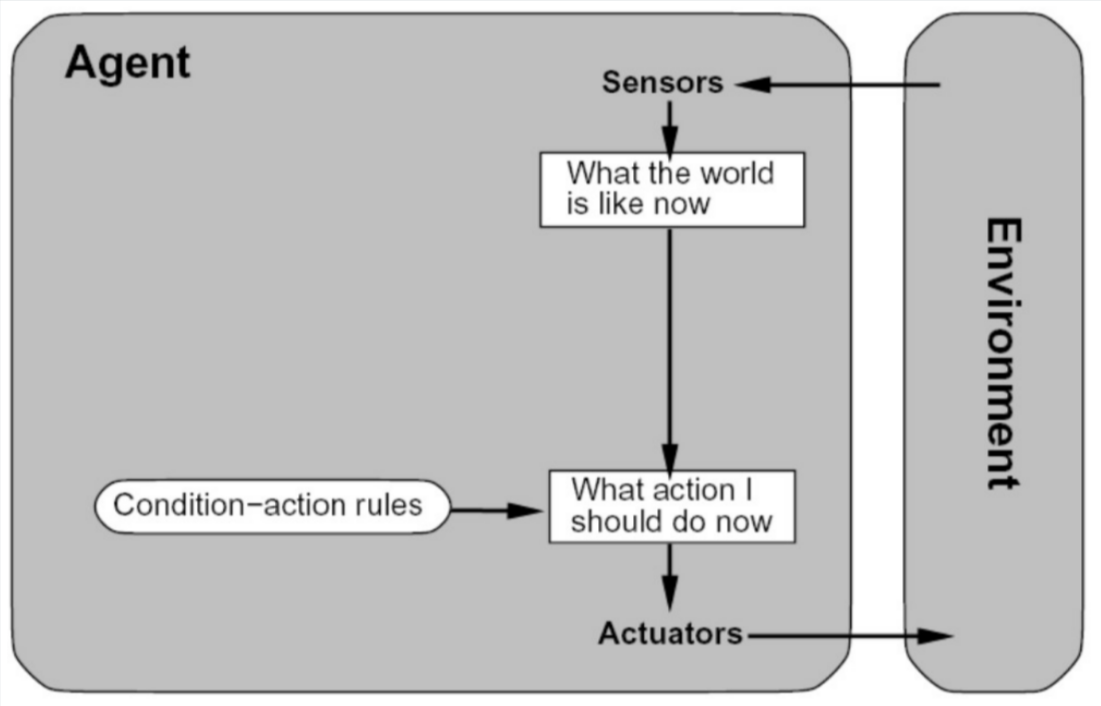
\includegraphics[width=16cm, scale=1]{Images/Imagenes/AgenteReflexoSimple.png}
  \caption{Agente reflexo simple}
\end{figure}

\subsubsection*{Agente reflexo con estado interno}
Tiene un estado interno que le permite
\begin{itemize}
  \item Ver como cambia el ambiente independientemente del agente
  \item Como afectan sus acciones al ambiente (osea tiene memoria)
\end{itemize}

\begin{figure}
  \centering
  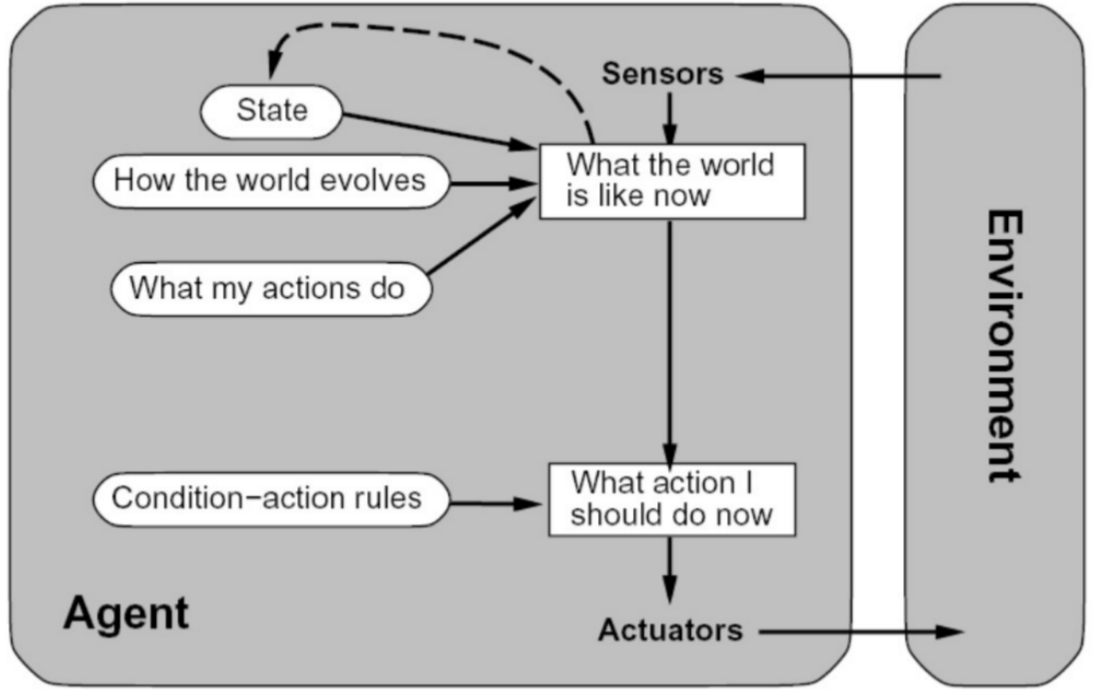
\includegraphics[width=16cm, scale=1]{Images/Imagenes/AgenteReflexoEst.png}
  \caption{Agente reflexo con estado interno}
\end{figure}

\subsubsection*{Agente orientado a metas}
\begin{itemize}
  \item Necesita información de sus metas para escoger que acciones las pueden cumplir
  \item Pueden usarse técnicas de búsqueda y planificación
  \item Esto lo puede hacer mas flexible. Por ejemplo si esta lloviendo ajustar la efectividad de los frenos. Básicamente analiza que es lo que hacen (pero no evalua que tan buenas son) sus posibles acciones para decidir si lo acercan o no a su meta esto quiere decir que buscan un objetivo sin importarle el como (osea le chupa un huevo la eficiencia solo quiere cumplir su objetivo)
\end{itemize}

\begin{figure}
  \centering
  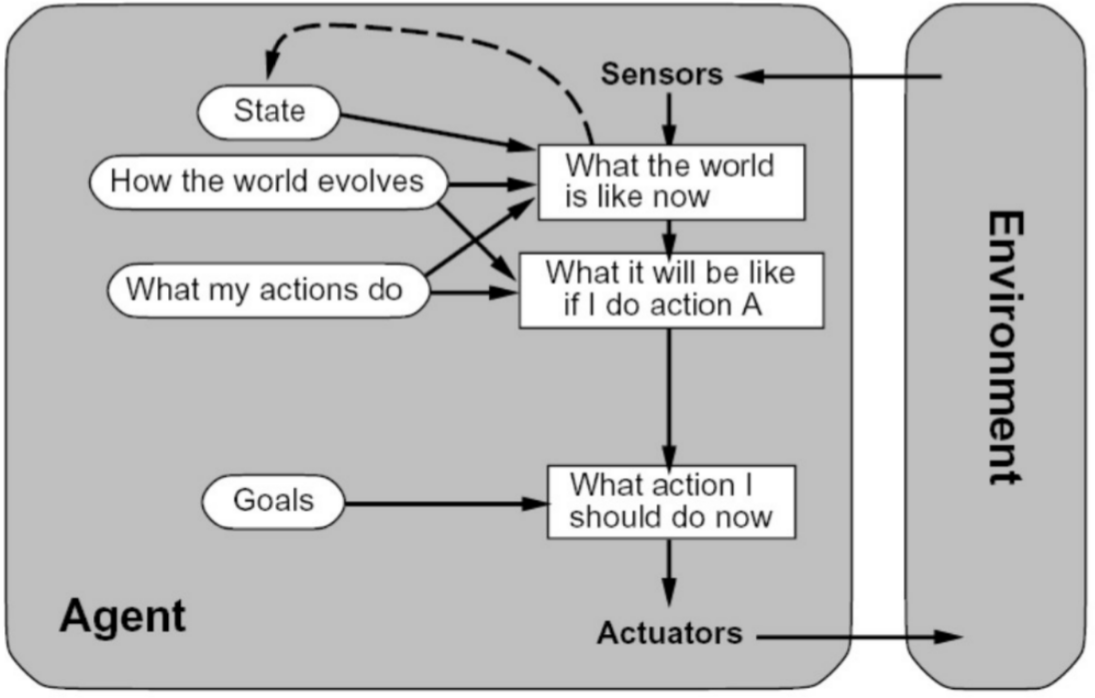
\includegraphics[width=16cm, scale=1]{Images/Imagenes/AgenteOrientadoAMetas.png}
  \caption{Agente orientado a metas}
\end{figure}

\subsubsection*{Agente orientado a la utilidad}
\begin{itemize}
  \item Las metas por si solas no son suficientes para generar un comportamiento de buena calidad (a este no le chupa un huevo la eficiencia :D)
  \item Para esto se necesita una medida de utilidad (función que mapea un estado o secuencia de estados con un numero real).básicamente tiene una función que le tira un numerito que dice que tan buena es la acción para ver si la toma o no.
\end{itemize}

\begin{figure}
  \centering
  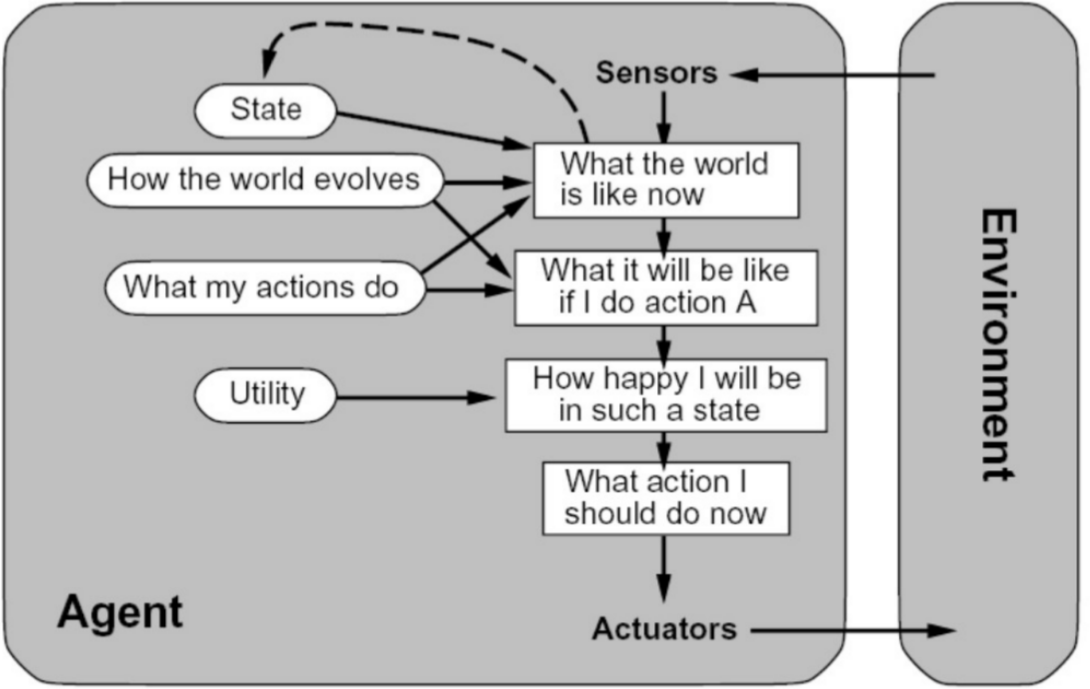
\includegraphics[width=16cm, scale=1]{Images/Imagenes/AgenteOrientadoAutilidad.png}
  \caption{Agente orientado a utilidad}
\end{figure}

\subsubsection*{Agentes que aprenden}
La idea es que las percepciones no se usen solo para actuar sino también para mejorar su desempeño en el futuro (osea es critico consigo mismo evalúa constantemente sus acciones y como afectaron al entorno buscando evolucionar y mejorar)

\begin{figure}
  \centering
  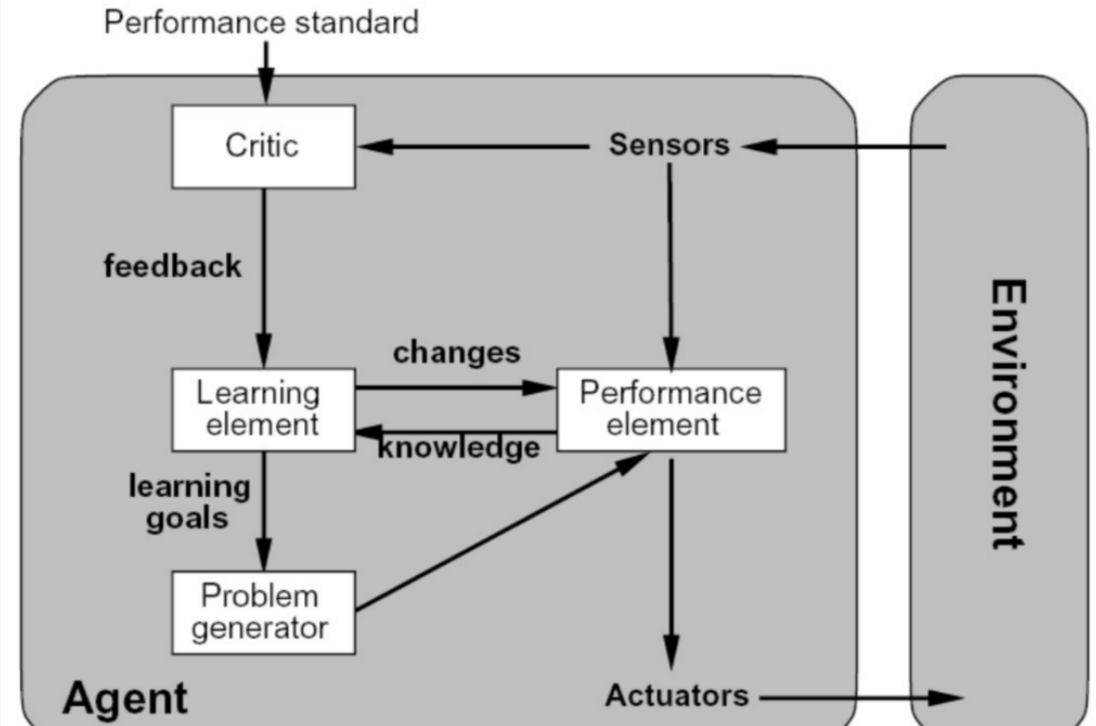
\includegraphics[width=16cm, scale=1]{Images/Imagenes/AgenteQueAprende.png}
  \caption{Agente que aprende}
\end{figure}

\subsubsection*{Inteligencia artificial distribuida-DAI}
\todo[inline]{esto da la sensacion de que no lo preguntan o que ni importa pero si con entender que es un sist. multiagente y como interactuan entre si alcanza}
Es el estudio construcción y aplicación de sistemas multiagente esto es sistemas en los cuales varios agentes inteligentes interactúan persiguiendo algún conjunto de objetivos o ejecutando algún conjunto de tareas. Un sistema multiagente es uno que consiste de un numero de agentes que interactúan entre ellos. En el caso mas general los agentes actúan en favor de sus usuarios con diferentes metas y motivaciones

\textbf{Como interactuan los agentes multiagente}
\begin{itemize}
  \item Coordinación: orientada a la meta o la tarea a realizar ej. cuando dos agentes requieren de un recurso.
  \item Cooperación: varios agentes tratan de combinar sus esfuerzos para lograr un objetivo en grupo. Ningún agente puede en forma solitaria lograr el objetivo o bien la cooperación hace obtener mejores resultados ej. obtener resultados en forma mas rápida
  \item Competición: varios agentes tratan de obtener lo que solo algunos de ellos pueden tener
  \item Negociación: varios agentes tratan de obtener su mayor beneficio logrando un acuerdo. Típicamente involucra una oferta contraoferta con compromisos hechos por los participantes 
\end{itemize}

\subsubsection*{Resumen de que es un agente inteligente}
Son entidades que:
\begin{itemize}
  \item perciben el ambiente
  \item actúan en el
  \item razonan
  \item se comunican con otros agentes
\end{itemize}
Es capaz de acciones autónomas flexibles es decir:
\begin{itemize}
  \item \textbf{Reactividad: }son capaces de percibir su ambiente y responde a cambios que ocurren
  \item \textbf{Pro-actividad: }son capaces de exhibir funcionamiento orientado a un objetivo tomando la iniciativa
  \item \textbf{Habilidad social: }son capaces de interactuar con otros agentes (o humanos)
\end{itemize}

\subsection*{Ambientes}
\subsubsection*{Completamente observable vs Parcialmente observable}

Un ambiente es completamente observable si los sensores del agente detectan todos los aspectos relevantes para decidir que acción debe llevarse a cabo. ej Poker seria parcialmente observable y Ajedrez completamente observable

\subsubsection*{Deterministico vs Estocastico}

Si el siguiente estado del ambiente esta completamente determinado por el estado actual y la acción ejecutada por el agente el ambiente es deterministico. Si otros factores influyen en el proximo estado del ambiente este es estocástico. ej. jugando al ajedrez el proximo estado del ambiente va a estar determinado por el estado actual y la pieza que se elija mover. Jugando a los dados no esta determinado el proximo estado del ambiente por la acción que realice el agente u el estado actual del ambiente (hay un factor aleatorio que afecta) por lo tanto es estocástico.

\subsubsection*{Agente único vs multiagente}

Un ambiente multiagente es un contexto en el cual multiples agentes interaccionan entre si con su entorno. En un agente único hay un solo agente que toma decisiones y realiza acciones sobre el entorno 

Los ambientes multiagente pueden ser los nombrados mas arriba

\subsubsection*{Episódico vs Secuencial}
En un ambiente episódico la experiencia del agente esta dividida en episodios atómicos. En cada episodio el agente percibe y ejecuta una acción simple y el siguiente episodio no depende de las acciones tomadas en episodios anteriores. Ej. Girar una ruleta seria episódico ya que el ambiente no se va a ver afectado por las tiradas anteriores solo por la acción. Mover una pieza en ajedrez seria secuencial ya que el nuevo estado depende de las acciones realizadas previamente

\subsubsection*{Discreto vs Continuo}
Esta distinción se aplica al estado del ambiente al modo en que se maneja el tiempo y a las percepciones y acciones del agente. ej. el tablero de ajedrez es un ambiente discreto. Cada casilla del tablero representa una posición única y hay un numero finito y discreto de piezas en juego. Cada movimiento del juego es una acción discreta ya que el agente selecciona una casilla especifica para mover una pieza. Un robot manipulador industrial trabaja en un ambiente continuo ya que puede mover su brazo y herramienta en una gama infinita de posiciones y orientaciones en el espacio tridimensional. Las acciones para controlar el robot se realizan de manera continua

\subsubsection*{Conocido vs No conocido}
Se refiere mas al estado de conocimiento del agente sobre las leyes o reglas del ambiente. Diferente de parcial-completamente observable. Ej. el solitario es parcialmente observable pero conozco las reglas por lo tanto es conocido

\section{Representación del conocimiento}
\todo[inline]{Resumi fuertemente, ni creo que entre pero si preguntan algo va a ser esto}
Es el area de la IA que se encarga de estudiar como describir el conocimiento del mundo o de un estado del mundo en forma simbólica. Estos símbolos luego son utilizados para representar una colección de proposiciones creídas por un agente. NO representamos TODO el conocimiento del agente, solamente definimos un conjunto finito luego con \textbf{razonamiento} achicamos la brecha entre lo representado y lo que el agente cree (osea obtenemos conocimiento de lo que el agente va a creer). 

En ciencias de la computación, una \textbf{ontología} representa formalmente el conocimiento como un conjunto de conceptos en un dominio y las relaciones entre estos conceptos. Asi se determina, que es lo que el agente puede percibir y por lo tanto, que parte del mundo va a representar y razonar a partir de los conceptos para lograr sus objetivos

\section{Agentes lógicos/IA simbólica}
\textbf{IA simbólica} El comportamiento inteligente puede ser generado en un sistema dándole al mismo: una representación simbólica de su ambiente y su comportamiento deseado y manipulando esta representación 

En IA, el proceso de obtener inteligencia o aprender corresponde a los agentes basados en conocimiento estos pueden
\begin{itemize}
  \item Pueden aceptar nuevas tareas en forma de metas descritas explícitamente (osea hacer cosas nuevas)
  \item Pueden adquirir competencias rápidamente o aprender nuevo conocimiento del ambiente (osea aprender en función de como evoluciona el ambiente)
  \item Pueden adaptarse a cambios en el ambiente, actualizando el conocimiento relevante (lo mismo que el item de arriba)
\end{itemize}

\textbf{Base de conocimiento: }contiene toda la información relevante del mundo que queremos representar, consiste en: 
\begin{itemize}
  \item Es un conjunto de sentencias que representan hechos sobre el mundo
  \item Si no son inferidas a partir de otras sentencias son axiomas
  \item Las sentencias son expresadas en un lenguaje formal de representación de conocimiento
\end{itemize}

\section{Búsqueda: }
Un agente solucionador de problemas es un agente inteligente orientado a metas que resuelve los problemas considerando secuencias de acciones que logren su meta. Para estos agentes se tiene que:
\begin{itemize}
  \item La representación del conocimiento es atómica, es decir cada estado del mundo es indivisible
  \item Formulación de la meta: la meta ayuda a organizar el comportamiento limitando las acciones que necesita considerar
  \item Acciones disponibles y los efectos de estas acciones
  \item Entorno: Los diferentes tipos de ambientes
  \item El razonamiento se reduce a la elección de una acción de acuerdo al efecto que tiene
\end{itemize}

\textbf{Búsqueda: }Es el proceso de buscar una secuencia de acciones que alcance una meta

\textbf{Problema: }se puede definir a traves de los siguientes componentes:
\begin{itemize}
  \item \textbf{Estado inicial:} donde el agente comienza
  \item \textbf{Acciones:} Descripción de las acciones posibles que posee el agente desde un estado s.
  \item \textbf{Modelo de transición y estados sucesores:} Una descripción de lo que cada acción hace, básicamente devuelve el estado al que te lleva cada acción
  \item \textbf{Test de meta: }determina si un estado es un estado meta
  \item \textbf{Función de costo del camino: }asigna un costo numérico a cada camino.
\end{itemize}

Con el estado inicial, las acciones y la función del estado sucesor se define el espacio de búsqueda de un problema. El espacio de búsqueda forma ung grafo en donde los nodos son los estados y los arcos las acciones aplicables desde ese nodo. Un camino es una secuencia de estados conectados por una secuencia de acciones.

\textbf{Estrategias de búsqueda: }son evaluadas según las siguientes dimensiones:
\begin{itemize}
  \item \textbf{Completitud: }Garantiza encontrar una solución siempre y cuando exista
  \item \textbf{Optimalidad: }Garantiza encontrar siempre la solución de menor costo
  \item \textbf{Complejidad temporal: }Numero de nodos generados
  \item \textbf{Complejidad espacial: }Máximo numero de nodos en memoria
\end{itemize}

\textbf{Estrategias de busqueda ciega (ir a diapo para ver propiedades, ni creo que pregunten igual): }
\begin{itemize}
  \item \textbf{Breadth-first: }Expande los nodos no expandidos mas cercanos (expande por nivel)
  \item \textbf{Depth-first: }Expande los nodos no expandidos mas profundos (osea va expandiendo hacia la izquierda al fondo y luego va subiendo por los nodos mas profundos que encuentre, si encuentra uno sin expandir lo expande y baja por la izquierda al fondo otra vez)
  \item \textbf{Depth-limited: }Lo mismo que Depth-first pero se pone un limite de profundidad l. Osea los nodos de profunidad l no se expanden, aun teniendo sucesores
\end{itemize}

\section{Búsqueda heurística}
La búsqueda ciega realiza un recorrido exhaustivo del árbol de búsqueda. Son independientes del problema que queremos resolver. Aun en problemas de espacios finitos, resultan de poco interés cuando el espacio es muy grande 

\textbf{Heurística: }Reglas para elegir o buscar las ramas en el espacio de estados que son más probables de llegar a una solución aceptable del problema. Son criterios que pueden resolver un problema pero que no hay garantía de que siempre lo resuelva. Básicamente la heurística informa a la búsqueda sobre qué dirección tomar para llegar a la meta. Provee un modo informado de adivinar cuál vecino de un nodo nos guía a la meta

\textbf{Costo real: }Sería el costo mas chico/óptimo para llegar a la solución

\textbf{Heurística admisible: }Es aquella que subestima el costo. Osea la estimación que realiza es menor o igual al costo real. Si g es el costo real de llegar desde el nodo actual a la meta entonces h <= g 

\textbf{Heurística mejor: }si h2(n) >= h1(n) para todo n \textbf{(ambas heurísticas admisibles)} entonces h2 domina a h1 y es mejor para la búsqueda


\section{Lógica no monotonica}
Ningún lenguaje puede expresar todo el conocimiento sobre el entorno, un conjunto de formulas es solo una aproximación. Una regla que es general esta sujeta a una seria (infinita) de restricciones que no pueden ser codificadas. El principal problema de la lógica clásica es que las reglas de inferencia son adecuadas, es decir, los teoremas son validos en todos los modelos de la base de conocimiento (no descartan modelos no deseados; no refinan). Las reglas de inferencia solo hacen explicito conocimiento que estaba implícito en la base de conocimiento. Por lo tanto la lógica clásica solo utiliza hechos que son eternamente verdaderos o eternamente falsos. No puede tratar ni la incertidumbre ni la revision

La logica clasica es \textbf{monotonica} y por lo tanto es:
\begin{itemize}
  \item \textbf{Muy debil: }No permite derivar lo que se intuye
  \item \textbf{Muy fuerte: }deriva todo el lenguaje frente a inconsistencias (osea en ningún momento hace revisiones sobre su conocimiento)
\end{itemize}

\section{Planning} 
Permite abrir la representación de las acciones y las metas para permitir la selección. Ademas permite dividir y conquistar descomponiendo el problema en submetas y relajar los requerimientos de construcción secuencial de soluciones.

Es una técnica en inteligencia artificial (IA) que se utiliza para la toma de decisiones secuenciales en un entorno. Implica la generación de secuencias de acciones que permiten alcanzar un objetivo específico, teniendo en cuenta el estado actual del entorno y las posibles acciones disponibles. 

Por otro lado, la búsqueda en IA se refiere a la exploración de un espacio de posibles soluciones para un problema. Se utiliza para encontrar una solución óptima o satisfactoria a un problema, pero no necesariamente implica la planificación de una secuencia de acciones. 

La principal diferencia radica en que el planning se enfoca en la planificación de acciones secuenciales para lograr un objetivo específico, mientras que la búsqueda en IA se centra en encontrar soluciones en un espacio de posibilidades, que puede o no incluir la planificación de acciones.

\subsection{STRIPS}
Su objetivo principal es encontrar una secuencia de acciones que permitan transformar un estado inicial del mundo en un estado objetivo.

Las características clave de STRIPS son las siguientes:

\begin{enumerate}
  \item \textbf{Representación del mundo: }En STRIPS, el mundo se representa como un conjunto de estados y operadores. Los estados son descripciones del mundo en un momento dado, y los operadores representan las acciones que se pueden llevar a cabo para cambiar de un estado a otro.
  \item \textbf{Estado inicial y objetivo:} Se define un estado inicial que representa el punto de partida del problema y un estado objetivo que representa el resultado deseado. El objetivo del sistema es encontrar una secuencia de operadores que lleven del estado inicial al estado objetivo
  \item \textbf{Precondiciones y efectos:}  Cada operador tiene precondiciones que deben ser verdaderas en el estado actual para que se pueda aplicar la operación. Además, cada operador tiene efectos que indican cómo cambiarán las condiciones del mundo una vez que se aplique la operación.
  \item \textbf{Planificación:} STRIPS utiliza algoritmos de planificación para buscar la secuencia de operadores que transformarán el estado inicial en el estado objetivo. Los algoritmos de planificación en STRIPS pueden incluir la búsqueda en profundidad, búsqueda en amplitud y búsqueda heurística.
\end{enumerate}

Proporciona una forma estructurada de representar el mundo, las acciones y los objetivos, lo que permite a los sistemas de inteligencia artificial encontrar secuencias de acciones que logren un resultado deseado. 

\subsection{Situation Calculus}
Proporciona una forma estructurada de razonar sobre cómo cambia el mundo a medida que se ejecutan acciones. Aquí están los aspectos clave del Cálculo de Situaciones:

\begin{enumerate}
  \item \textbf{Situaciones: }En el Cálculo de Situaciones, un "situation" (situación) es una descripción de un estado del mundo en un momento dado. Estas situaciones representan cómo se ve el mundo en un punto específico en el tiempo. Puedes pensar en una situación como una instantánea que captura todos los hechos relevantes sobre el estado actual del mundo.
  \item \textbf{Acciones: }Las acciones son operadores que transforman una situación en otra. Representan cómo el mundo cambia como resultado de una acción específica. Cada acción tiene precondiciones que deben ser ciertas en una situación antes de que se pueda ejecutar. Además, cada acción tiene efectos que indican cómo cambian las condiciones del mundo después de que se ha ejecutado.
  \item \textbf{Operadores de Transición: }En el Cálculo de Situaciones, se utilizan operadores de transición para describir cómo una situación se relaciona con otra a través de una acción. Estos operadores se utilizan para modelar cómo se pasa de una situación a la siguiente mediante la ejecución de una acción. Los operadores de transición conectan situaciones actuales con situaciones resultantes.
  \item \textbf{Lógica Temporal: }El Cálculo de Situaciones a menudo se combina con lógica temporal para razonar sobre secuencias de acciones a lo largo del tiempo. Esto permite modelar y razonar sobre eventos que ocurren en secuencia y cómo afectan al estado del mundo. 
\end{enumerate}

Permite a los sistemas de inteligencia artificial modelar y predecir cómo cambiará el mundo a medida que se ejecutan acciones, lo que es fundamental en tareas de planificación, robótica y toma de decisiones en tiempo real lo que lo convierte en una herramienta poderosa en la inteligencia artificial y la filosofía para modelar y comprender situaciones dinámicas.


\subsection{Event Calculus}
El Cálculo de Eventos (Event Calculus) es un formalismo lógico utilizado en la inteligencia artificial y la representación del conocimiento para modelar y razonar sobre eventos y su evolución en un dominio específico: 

\begin{enumerate}
  \item \textbf{Eventos: }En el Cálculo de Eventos, el mundo se describe en términos de eventos. Un evento es una ocurrencia que afecta al estado del mundo. Puede ser cualquier cosa, desde una acción específica hasta un cambio en una condición, y se representa de manera lógica. Los eventos se utilizan para capturar cambios en el mundo a lo largo del tiempo.
  \item \textbf{Fluentes: }Los fluents (conceptos fluídos) son propiedades o predicados que pueden ser verdaderos o falsos en un momento dado. Los eventos pueden causar cambios en los fluents. Por ejemplo, un fluent ``puerta\_abierta'' puede cambiar de ``verdadero'' a ``falso'' como resultado del evento ``abrir\_puerta''.
  \item \textbf{Efectos Temporales: }El Cálculo de Eventos también tiene en cuenta efectos temporales. Los eventos pueden tener una duración o un periodo de validez. Esto permite modelar eventos que ocurren durante un período de tiempo en lugar de en un punto único.
  \item \textbf{Reglas de Evento: }Se utilizan reglas de evento para representar cómo los eventos afectan a los fluents y al estado del mundo. Estas reglas describen las condiciones bajo las cuales un evento causa un cambio en un fluent y cómo se produce ese cambio.
  \item \textbf{Historia del Mundo: }El Cálculo de Eventos mantiene un registro de la historia del mundo en términos de eventos y sus efectos en los fluents. Esto permite razonar retroactivamente sobre eventos pasados y predecir eventos futuros.
  \item \textbf{Razonamiento Temporal: }Una de las aplicaciones clave del Cálculo de Eventos es el razonamiento temporal. Permite responder preguntas como ``¿Qué fluents eran verdaderos en un momento específico?'' o ``¿Cuándo ocurrirá un evento particular?''.
  \item \textbf{Planificación y Toma de Decisiones: }El Event Calculus se utiliza en planificación y toma de decisiones en entornos dinámicos. Puede ayudar a los sistemas de inteligencia artificial a planificar y ejecutar secuencias de acciones considerando cómo los eventos afectan al estado del mundo a lo largo del tiempo.
\end{enumerate}

El Cálculo de Eventos es un formalismo lógico que se centra en la representación y el razonamiento sobre eventos y su impacto en el estado del mundo a lo largo del tiempo. Es especialmente útil para modelar entornos dinámicos y razonar sobre eventos pasados y futuros, lo que lo convierte en una herramienta poderosa en campos como la robótica, la planificación, la toma de decisiones y la representación del conocimiento en inteligencia artificial.

\subsection{Ejemplos de uso}
\textbf{STRIPS}
\begin{itemize}
  \item \textbf{Ejemplo:} Planificación de un robot para ensamblar un producto en una cadena de montaje.
  \item \textbf{Razón de elección:} STRIPS es ideal para problemas de planificación en los que se requiere una secuencia de acciones para alcanzar un objetivo específico. En este caso, planificar las acciones del robot para ensamblar un producto en un orden específico es una tarea secuencial que se adapta bien al enfoque de STRIPS.
\end{itemize}

\textbf{Situation Calculus: }
\begin{itemize}
  \item \textbf{Ejemplo:} Modelado de un sistema de juego de ajedrez donde se necesita razonar sobre el estado del tablero y las posibles jugadas.
  \item \textbf{Razón de elección:} El Cálculo de Situaciones es útil cuando se necesita razonar sobre cómo cambian las situaciones a lo largo del tiempo debido a eventos y acciones. En el ajedrez, se pueden modelar los movimientos de las piezas como eventos que cambian el estado del tablero, lo que hace que el Cálculo de Situaciones sea apropiado.
\end{itemize}

\textbf{Event Calculus:}
\begin{itemize}
  \item \textbf{Ejemplo:} Modelado de un sistema de supervisión de la salud de un paciente en un hospital, donde es importante rastrear eventos como medicamentos administrados y cambios en las condiciones del paciente.
  \item \textbf{Razón de elección:} El Cálculo de Eventos se adapta a escenarios en los que se necesita rastrear y razonar sobre eventos que afectan el estado del mundo a lo largo del tiempo. En el caso del monitoreo de la salud del paciente, los eventos (administración de medicamentos, cambios en la condición) tienen un impacto en el estado del paciente, lo que hace que el Cálculo de Eventos sea una elección adecuada.
\end{itemize}

La elección entre estos enfoques depende de la naturaleza del problema y cómo se necesita representar y razonar sobre eventos y cambios en el mundo. STRIPS es adecuado para problemas de planificación secuencial, el Cálculo de Situaciones es útil para razonar sobre cambios a lo largo del tiempo debido a eventos, y el Cálculo de Eventos es valioso cuando se necesita un seguimiento y razonamiento detallado sobre eventos y sus efectos. La elección dependerá de los requisitos específicos del dominio y del problema que se está abordando.
